
%-----------------------------------------------------------------------------------------------------------------------------------------------%
%	The MIT License (MIT)
%
%	Copyright (c) 2019 Jan Küster
%
%	Permission is hereby granted, free of charge, to any person obtaining a copy
%	of this software and associated documentation files (the "Software"), to deal
%	in the Software without restriction, including without limitation the rights
%	to use, copy, modify, merge, publish, distribute, sublicense, and/or sell
%	copies of the Software, and to permit persons to whom the Software is
%	furnished to do so, subject to the following conditions:
%
%	THE SOFTWARE IS PROVIDED "AS IS", WITHOUT WARRANTY OF ANY KIND, EXPRESS OR
%	IMPLIED, INCLUDING BUT NOT LIMITED TO THE WARRANTIES OF MERCHANTABILITY,
%	FITNESS FOR A PARTICULAR PURPOSE AND NONINFRINGEMENT. IN NO EVENT SHALL THE
%	AUTHORS OR COPYRIGHT HOLDERS BE LIABLE FOR ANY CLAIM, DAMAGES OR OTHER
%	LIABILITY, WHETHER IN AN ACTION OF CONTRACT, TORT OR OTHERWISE, ARISING FROM,
%	OUT OF OR IN CONNECTION WITH THE SOFTWARE OR THE USE OR OTHER DEALINGS IN
%	THE SOFTWARE.
%
%
%-----------------------------------------------------------------------------------------------------------------------------------------------%


%============================================================================%
%
%	DOCUMENT DEFINITION
%
%============================================================================%

\documentclass[10pt,A4,english]{article}


%----------------------------------------------------------------------------------------
%	ENCODING
%----------------------------------------------------------------------------------------

% we use utf8 since we want to build from any machine
\usepackage[utf8]{inputenc}
\usepackage[USenglish]{isodate}
\usepackage{fancyhdr}
% \usepackage[numbers]{natbib}

%----------------------------------------------------------------------------------------
%	LOGIC
%----------------------------------------------------------------------------------------

% provides \isempty test
\usepackage{xstring, xifthen}
\usepackage{enumitem}
\usepackage[english]{babel}
\usepackage{blindtext}
\usepackage{pdfpages}
\usepackage{changepage}
%----------------------------------------------------------------------------------------
%	FONT BASICS
%----------------------------------------------------------------------------------------

% some tex-live fonts - choose your own
\usepackage[default]{raleway}

% set font default
\renewcommand*\familydefault{\sfdefault}
\usepackage[T1]{fontenc}

% more font size definitions
\usepackage{moresize}

%----------------------------------------------------------------------------------------
%	FONT AWESOME ICONS
%----------------------------------------------------------------------------------------

% include the fontawesome icon set
\usepackage{fontawesome5}

% use to vertically center content
% credits to: http://tex.stackexchange.com/questions/7219/how-to-vertically-center-two-images-next-to-each-other
\newcommand{\vcenteredinclude}[1]{\begingroup
\setbox0=\hbox{\includegraphics{#1}}%
\parbox{\wd0}{\box0}\endgroup}
\newcommand{\tab}[1]{\hspace{.2\textwidth}\rlap{#1}}
% use to vertically center content
% credits to: http://tex.stackexchange.com/questions/7219/how-to-vertically-center-two-images-next-to-each-other
\newcommand*{\vcenteredhbox}[1]{\begingroup
\setbox0=\hbox{#1}\parbox{\wd0}{\box0}\endgroup}

% icon shortcut
\newcommand{\icon}[2] {
	\makebox(#2, #2){\textcolor{maincol}{\textcolor{maincol}{\faIcon{#1}}}}
}


% icon with text shortcut
\newcommand{\icontext}[3]{
	\vcenteredhbox{\icon{#1}{#2}}  \hspace{2pt}  \parbox{0.9\mpwidth}{\textcolor{black}{#3}}
}

% icon with website url
\newcommand{\iconhref}[4]{
    \vcenteredhbox{\icon{#1}{#2}}  \hspace{2pt} \href{#4}{\textcolor{black}{#3}}
}

% icon with email link
\newcommand{\iconemail}[5]{
    \vcenteredhbox{\icon{#1}{#2}{#5}}  \hspace{2pt} \href{mailto:#4}{\textcolor{#5}{#3}}
}

%----------------------------------------------------------------------------------------
%	PAGE LAYOUT  DEFINITIONS
%----------------------------------------------------------------------------------------

% page outer frames (debug-only)
% \usepackage{showframe}

% we use paracol to display breakable two columns
\usepackage{paracol}
\usepackage{tikzpagenodes}
\usetikzlibrary{calc}
\usepackage{lmodern}
\usepackage{multicol}
\usepackage{lipsum}
\usepackage{atbegshi}
% define page styles using geometry
\usepackage[a4paper]{geometry}

% remove all possible margins
\geometry{top=1cm, bottom=1cm, left=1cm, right=1cm}

\usepackage{fancyhdr}
\pagestyle{empty}

% space between header and content
% \setlength{\headheight}{0pt}

% indentation is zero
\setlength{\parindent}{0mm}

%----------------------------------------------------------------------------------------
%	TABLE /ARRAY DEFINITIONS
%----------------------------------------------------------------------------------------

% extended aligning of tabular cells
\usepackage{array}

% custom column right-align with fixed width
% use like p{size} but via x{size}
\newcolumntype{x}[1]{%
>{\raggedleft\hspace{0pt}}p{#1}}%


%----------------------------------------------------------------------------------------
%	GRAPHICS DEFINITIONS
%----------------------------------------------------------------------------------------

%for header image
\usepackage{graphicx}

% use this for floating figures
% \usepackage{wrapfig}
% \usepackage{float}
% \floatstyle{boxed}
% \restylefloat{figure}

%for drawing graphics
\usepackage{tikz}
\usepackage{ragged2e}
\usetikzlibrary{shapes, backgrounds,mindmap, trees}

%----------------------------------------------------------------------------------------
%	Bibliography
%----------------------------------------------------------------------------------------

%----------------------------------------------------------------------------------------
%	Color DEFINITIONS
%----------------------------------------------------------------------------------------
\usepackage{transparent}
\usepackage{color}

% primary color
\definecolor{maincol}{RGB}{0, 0, 128}

% accent color, secondary
% \definecolor{accentcol}{RGB}{ 250, 150, 10 }

% dark color
\definecolor{darkcol}{RGB}{ 70, 70, 70 }

% light color
\definecolor{lightcol}{RGB}{245,245,245}

\definecolor{accentcol}{RGB}{0, 0, 128}



% Package for links, must be the last package used
\usepackage[hidelinks]{hyperref}

% returns minipage width minus two times \fboxsep
% to keep padding included in width calculations
% can also be used for other boxes / environments
\newcommand{\mpwidth}{\linewidth-\fboxsep-\fboxsep}



%============================================================================%
%
%	CV COMMANDS
%
%============================================================================%

%----------------------------------------------------------------------------------------
%	 CV LIST
%----------------------------------------------------------------------------------------

% renders a standard latex list but abstracts away the environment definition (begin/end)
\newcommand{\cvlist}[1] {
	\begin{itemize}{#1}\end{itemize}
}

%----------------------------------------------------------------------------------------
%	 CV TEXT
%----------------------------------------------------------------------------------------

% base class to wrap any text based stuff here. Renders like a paragraph.
% Allows complex commands to be passed, too.
% param 1: *any
\newcommand{\cvtext}[1] {
	\begin{tabular*}{1\mpwidth}{p{0.98\mpwidth}}
		\parbox{1\mpwidth}{#1}
	\end{tabular*}
}
\newcommand{\cvtextsmall}[1] {
	\begin{tabular*}{0.8\mpwidth}{p{0.8\mpwidth}}
		\parbox{0.8\mpwidth}{#1}
	\end{tabular*}
}
%----------------------------------------------------------------------------------------
%	CV SECTION
%----------------------------------------------------------------------------------------

% Renders a a CV section headline with a nice underline in main color.
% param 1: section title
\newlength{\barw}
\newcommand{\cvsection}[1] {
	\vspace{14pt}
	\settowidth{\barw}{\textbf{\LARGE #1}}
	\cvtext{
		\textbf{\LARGE{\textcolor{darkcol}{#1}}}\\[-4pt]
		\textcolor{accentcol}{ \rule{\barw}{1.5pt} } \\
	}
}

\newcommand{\cvsubsection}[1] {
	\vspace{14pt}
	\settowidth{\barw}{\textbf{\Large #1}}
	\cvtext{
		\textbf{\Large{\textcolor{darkcol}{#1}}}\\[-4pt]
		\textcolor{accentcol}{ \rule{\barw}{1.5pt} } \\
	}
}

\newcommand{\cvheadline}[1] {
	\vspace{16pt}
	\cvtext{
		\textbf{\Huge{\textcolor{accentcol}{#1}}}\\[-4pt]

	}
}

\newcommand{\cvsubheadline}[1] {
	\vspace{16pt}
	\cvtext{
		\textbf{\huge{\textcolor{darkcol}{#1}}}\\[-4pt]

	}
}
%----------------------------------------------------------------------------------------
%	META SKILL
%----------------------------------------------------------------------------------------

% Renders a progress-bar to indicate a certain skill in percent.
% param 1: name of the skill / tech / etc.
% param 2: level (for example in years)
% param 3: percent, values range from 0 to 1
\newcommand{\cvskill}[3] {
	\begin{tabular*}{1\mpwidth}{p{0.72\mpwidth}  r}
 		\textcolor{black}{\textbf{#1}} & \textcolor{maincol}{#2}\\
	\end{tabular*}%

	\hspace{4pt}
	\begin{tikzpicture}[scale=1,rounded corners=2pt,very thin]
		\fill [lightcol] (0,0) rectangle (1\mpwidth, 0.15);
		\fill [accentcol] (0,0) rectangle (#3\mpwidth, 0.15);
  	\end{tikzpicture}%
}


%----------------------------------------------------------------------------------------
%	 CV EVENT
%----------------------------------------------------------------------------------------

% Renders a table and a paragraph (cvtext) wrapped in a parbox (to ensure minimum content
% is glued together when a pagebreak appears).
% Additional Information can be passed in text or list form (or other environments).
% the work you did
% param 1: time-frame i.e. Sep 14 - Jan 15 etc.
% param 2:	 event name (job position etc.)
% param 3: Customer, Employer, Industry
% param 4: Short description
% param 5: work done (optional)
% param 6: technologies include (optional)
% param 7: achievements (optional)
\newcommand{\cvevent}[4] {

	% we wrap this part in a parbox, so title and description are not separated on a pagebreak
	% if you need more control on page breaks, remove the parbox
	\parbox{\mpwidth}{
		\begin{tabular*}{1\mpwidth}{p{0.66\mpwidth}  r}
	 		\textcolor{black}{\textbf{#2}} & \colorbox{accentcol}{\makebox[0.32\mpwidth]{\textcolor{white}{\textbf{#1}}}} \\
			\textcolor{maincol}{#3} & \\
		\end{tabular*}\\[2pt]

		\ifthenelse{\isempty{#4}}{}{
			\cvtext{#4}\\
		}
	}
	\vspace{14pt}
}

\newcommand{\cvproj}[3] {
	\parbox{\mpwidth}{
		\begin{tabular*}{1\mpwidth}{p{0.66\mpwidth}  r}
	 		\textcolor{black}{\textbf{#1}} & \\
			\textcolor{maincol}{#2} & \\
		\end{tabular*}\\[4pt]

		\ifthenelse{\isempty{#3}}{}{
			\cvtext{#3}\\
		}
	}
	\vspace{14pt}
}

%----------------------------------------------------------------------------------------
%	 CV META EVENT
%----------------------------------------------------------------------------------------

% Renders a CV event on the sidebar
% param 1: title
% param 2: subtitle (optional)
% param 3: customer, employer, etc,. (optional)
% param 4: info text (optional)
\newcommand{\cvmetaevent}[4] {
	\textcolor{maincol} { \cvtext{\textbf{\begin{flushleft}#1\end{flushleft}}}}

	\ifthenelse{\isempty{#2}}{}{
	\textcolor{black} {\cvtext{\textbf{#2}} }
	}

	\ifthenelse{\isempty{#3}}{}{
		\cvtext{{ \textcolor{maincol} {#3} }}\\
	}

	\cvtext{#4}\\[14pt]
}

%---------------------------------------------------------------------------------------
%	QR CODE
%----------------------------------------------------------------------------------------

% Renders a qrcode image (centered, relative to the parentwidth)
% param 1: percent width, from 0 to 1
\newcommand{\cvqrcode}[1] {
	\begin{center}
		\includegraphics[width={#1}\mpwidth]{qrcode}
	\end{center}
}


% HEADER AND FOOOTER
%====================================
\newcommand\Header[1]{%
\begin{tikzpicture}[remember picture,overlay]
\fill[accentcol]
  (current page.north west) -- (current page.north east) --
  ([yshift=50pt]current page.north east|-current page text area.north east) --
  ([yshift=50pt,xshift=-3cm]current page.north|-current page text area.north) --
  ([yshift=10pt,xshift=-5cm]current page.north|-current page text area.north) --
  ([yshift=10pt]current page.north west|-current page text area.north west) -- cycle;
\node[font=\sffamily\bfseries\color{white},anchor=west,
  xshift=0.7cm,yshift=-0.32cm] at (current page.north west)
  {\fontsize{12}{12}\selectfont {#1}};
\end{tikzpicture}%
}

\newcommand\Footer[1]{%
\begin{tikzpicture}[remember picture,overlay]
\fill[lightcol]
  (current page.south east) -- (current page.south west) --
  ([yshift=-80pt]current page.south east|-current page text area.south east) --
  ([yshift=-80pt,xshift=-6cm]current page.south|-current page text area.south) --
  ([xshift=-2.5cm,yshift=-10pt]current page.south|-current page text area.south) --
  ([yshift=-10pt]current page.south east|-current page text area.south east) -- cycle;
\node[yshift=0.32cm,xshift=9cm] at (current page.south) {\fontsize{10}{10}\selectfont \textbf{\thepage}};
\end{tikzpicture}%
}


%=====================================
%============================================================================%
%
%
%
%	DOCUMENT CONTENT
%
%
%
%============================================================================%
\begin{document}

\columnratio{0.31}
\setlength{\columnsep}{2.2em}
\setlength{\columnseprule}{4pt}
\colseprulecolor{white}


% LEBENSLAUF HIERE
\AtBeginShipoutFirst{\Header{CV}\Footer{1}}
\AtBeginShipout{\AtBeginShipoutAddToBox{\Header{CV}\Footer{2}}}

\newpage

\colseprulecolor{lightcol}
\columnratio{0.31}
\setlength{\columnsep}{2.2em}
\setlength{\columnseprule}{4pt}
\begin{paracol}{2}
	\begin{leftcolumn}
		%---------------------------------------------------------------------------------------
		%	META IMAGE
		%----------------------------------------------------------------------------------------
		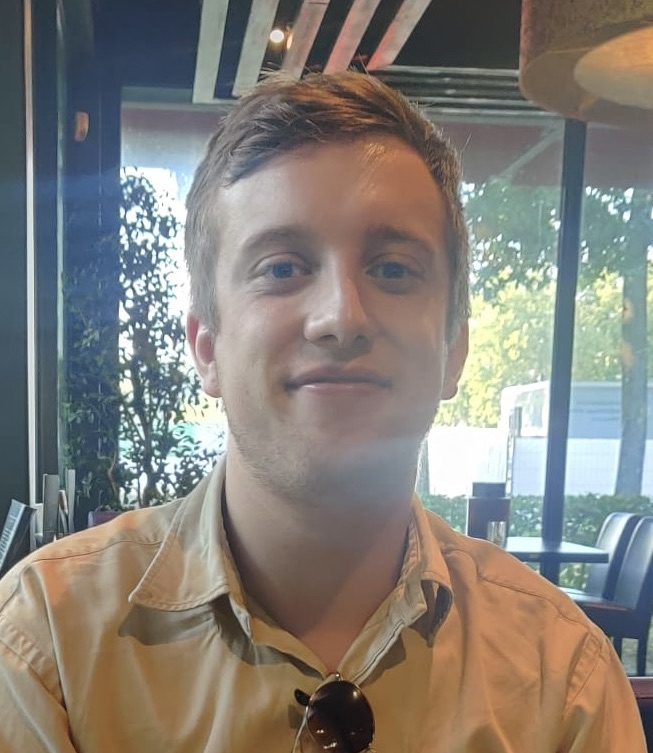
\includegraphics[width=\linewidth]{profile.jpg}
		\fcolorbox{white}{white}{\begin{minipage}[c][1.5cm][c]{1\mpwidth}
				\LARGE{\textbf{\textcolor{maincol}{Pepijn A. Vink}}} \\[2pt]
				\normalsize{ \textcolor{maincol} {MSc Student Methodology and
Statistics} }
			\end{minipage}}

		%---------------------------------------------------------------------------------------
		%	META SKILLS
		%----------------------------------------------------------------------------------------
				\icontext{caret-right}{12}{Pragmatic Bayesian}\\[6pt]
		
		
		\cvsection{Skills}

						\cvskill{R}{}{0.7} \\[10pt]
								\cvskill{Quarto}{}{0.55} \\[10pt]
								\cvskill{R Package Development}{}{0.3} \\[10pt]
								\cvskill{SPSS}{}{0.6} \\[10pt]
								\cvskill{JASP}{}{0.55} \\[10pt]
								\cvskill{JAGS}{}{0.2} \\[10pt]
								\cvskill{MPlus}{}{0.3} \\[10pt]
								\cvskill{GitHub}{}{0.5} \\[10pt]
								\cvskill{Teaching}{}{0.45} \\[10pt]
						
		\cvsection{Interests}

						\icontext{caret-right}{12}{Bayesian Statistics}\\[6pt]
								\icontext{caret-right}{12}{Longitudinal Data}\\[6pt]
								\icontext{caret-right}{12}{Bayesian Networks}\\[6pt]
								\icontext{caret-right}{12}{Open Science}\\[6pt]
						
		\cvsection{Contact}

						\icontext{map-marker}{16}{Utrecht, the Netherlands}\\[6pt]
								\icontext{envelope}{16}{p.a.vink@uu.nl}\\[6pt]
								\iconhref{linkedin}{16}{linkedin.nl/pepijnvink}{https://www.linkedin.com/in/pepijnvink/}\\[6pt]
								\iconhref{home}{16}{pepijnvink.github.io}{https://pepijnvink.github.io}\\[6pt]
								\iconhref{github}{16}{pepijnvink}{https://github.com/pepijnvink}\\[6pt]
								\iconhref{orcid}{16}{0000-0001-6960-9904}{https://orcid.org/0000-0001-6960-9904}\\[6pt]
						
	\end{leftcolumn}

	\begin{rightcolumn}
		\cvsection{Education} \vspace{4pt}

\cvevent{09/2022 - Present}{MSc Methodology and Statistics for the Behavioral, Biomedical, and Social Sciences (Research)}{Utrecht University}{\begin{itemize}\item Courses on multivariate statistics, survey data analysis, mathematical statistics, programming, Bayesian statistics, multilevel models, psychometrics, causal inference, structural equation modeling, markup languages, and data science.\item Thesis on implementation of causal inference methods in the Random Intercept Cross-Lagged Panel Model (supervised by prof. dr. Ellen Hamaker and Jeroen Mulder).\item Traineeship on Bayesian algorithms for structure learning of Bayesian networks (supervised by dr. Maarten Marsman and dr. Noémi Schuurman).\end{itemize}}

\cvevent{09/2019 - 07/2022}{BSc Psychology}{Utrecht University}{\begin{itemize}\item Specialization in Social Psychology. Average grade: 7.8.\item Thesis: Frequentism vs Bayesianism: A Conceptual and Quantitative Comparison of NHST, Confidence Intervals, Credible \newline Intervals, and the Bayes Factor Through Simulated t-tests (supervised by prof. dr. Irene Klugkist and Thijs Carrière). Grade: 8.5.\end{itemize}}

\cvevent{2010 - 2016}{VWO}{Christelijk Lyceum Zeist}{\begin{itemize}\item Specialized in natural sciences. Followed the bilingual education programme.\end{itemize}}

\cvsection{Experience} \vspace{4pt}

\cvevent{09/23 - Present}{Student Assistant Biostatistics Education}{UMC Utrecht}{\begin{itemize}\item Taught practicals for the courses ‘Classical Methods in Data Analysis (MSc Epidemiology)’ and ‘Epidemiology and Big Data (MSc Applied Data Science)’.\end{itemize}}

\cvevent{09/2021 - Present}{Student Assistant}{Utrecht University}{\begin{itemize}\item Teaching assistent for several bachelor courses for the faculty of social and behavioral sciences. This includes independently teaching workgroups as well as practicals for SPSS, JASP, R, and NVivo.\item Practical teacher for UU summer school courses on MPlus.\item Since September 2022 involved as a research assistant for Hanne Oberman. Tasks include programming for the {ggmice} package, preprocessing data, and working on a case study for a manuscript.\item Since November 2022 involved as a research assistant on the biennial Open Science Monitor.\end{itemize}}

\cvevent{2014-2019}{Side-jobs}{}{\begin{itemize}\item Supermarkt worker (2014-2016)\item Dishwasher at a restaurant (2016-2019)\item Sales employee at a shoe store (2019)\end{itemize}}

\cvsection{Extracurricular and Volunteering} \vspace{4pt}

\cvevent{09/2019 - 09/2020}{Vice-Praeses (Vice-President)}{U.H.S.V. Anteros}{\begin{itemize}\item U.H.S.V. Anteros is an LGBT+ Student Association in Utrecht.\item As Vice-President, I was mainly involved with maintaing relationships with other associations, occasionally chairing meetings, and supervising some committees, as well as other smaller tasks.\end{itemize}}

\cvevent{01/2018 - Present}{Member and Committee Member}{U.H.S.V. Anteros}{\begin{itemize}\item Committees include: travel committee, lustrum committee, themed drinks committee, party committee, internal regulations committee, and the selection committee for choosing the new board.\end{itemize}}

\cvevent{05/2020 - 05/2022}{Educator}{COC Midden-Nederland}{\begin{itemize}\item COC Midden-Nederland is a regional organization that advocates for LGBTI+ rights.\item As an educator, I taught guest lessons at high school on LGBTI+ experiences.\end{itemize}}

\cvsection{Conferences} \vspace{4pt}

\cvevent{09/11/2023}{Panel}{Conference for the International Scholarship of Teaching and Learning (ISOTL)}{\begin{itemize}\item Panel on the role of open science in teaching in higher education.\end{itemize}}
			\end{rightcolumn}
\end{paracol}


\end{document}
